%%%%% APPENDIX %%%%%%%%%%%%%%%%%%%%%%%%%%%%%%%%%%%%%%%%%%%%%%%%%%%%%%%
\appendix

\section{Interview Guideline} \label{section::interview_guideline}
\subsection{Interview Setup}
\begin{itemize}
    \item brief interviewee about thesis and their role in the research
    \item ask if the interview session may be recorded and further processed for scientific inquiry
    \item ensure technicalities before start of interview with participant:
    \begin{itemize}
        \item the participant's iPhone is sufficiently charged, has been restarted and is in "Do Not Disturb" mode
        \item the participant has installed Quicktime player on their iPhone and are sharing it with their MacBook
        \item the participant is sharing their MacBook screen in the video call
        \item the participant has received the QR codes for kickdown A and B
    \end{itemize}
    \item ask the participant if the recording may started
\end{itemize}

\subsection{Background Questions}
Ask the participant about their...
\begin{itemize}
    \item job role
    \item years of experience in the mobile app industry
    \item previous experience with the Kickdown application
\end{itemize}

\subsection{Main Interview}
\paragraph*{App Start and Scroll Behavior}\hfill \break
\textbf{Instructions}
\begin{itemize}
    \item Please open Kickdown (A/B) and find the [color] [brand] [attribute] car.
    \item Please open Kickdown (A/B) and find the [color] [brand] [attribute] car.
\end{itemize}

\textbf{Questions}
\begin{enumerate}
    \item Are there any differences in terms of user experience in any way between the two apps?
    \item If you had to pick one experience over the other, which would you choose (A or B)?
\end{enumerate}

\paragraph*{Detail Transition, Modal Transition, Textfield interaction}\hfill \break
\textbf{Instructions}
\begin{itemize}
    \item Please stay in Kickdown (A/B) and tap on a car of your choice. Bid on the car with an amount of your choice.
    \item Please repeat the process for the Kickdown (A/B). You may choose another car and enter a different amount.
\end{itemize}

\textbf{Questions}
\begin{enumerate}
    \item Are there any differences in terms of user experience in any way between the two apps?
    \item If you had to pick one experience over the other, which would you choose (A or B)?
\end{enumerate}


\paragraph*{Horizontal Scrolling}\hfill \break
\textbf{Instructions}
\begin{itemize}
    \item Please stay in Kickdown (A/B) and open the first posting. Find the picture with the [insert item].
    \item Please open Kickdown (A/B) and open the second posting. Find the picture with the [insert item].
\end{itemize}

\textbf{Questions}
\begin{enumerate}
    \item Are there any differences in terms of user experience in any way between the two apps?
    \item If you had to pick one experience over the other, which would you choose (A or B)?
\end{enumerate}

\paragraph*{    }\hfill \break
\textbf{Instructions}
\begin{itemize}
    \item Please stay in Kickdown (A/B) and use the tab navigation to navigate to the "More Screen". Please turn Tracking on.
    \item Please repeat the process for Kickdown (A/B)
\end{itemize}

\textbf{Questions}
\begin{enumerate}
    \item Are there any differences in terms of user experience in any way between the two apps?
    \item If you had to pick one experience over the other, which would you choose (A or B)?
\end{enumerate}


\section{Performance Result Graphs} \label{section::performance_tracing_results}

\subsection{App Start}

\begin{figure}[!h]
    \centering
    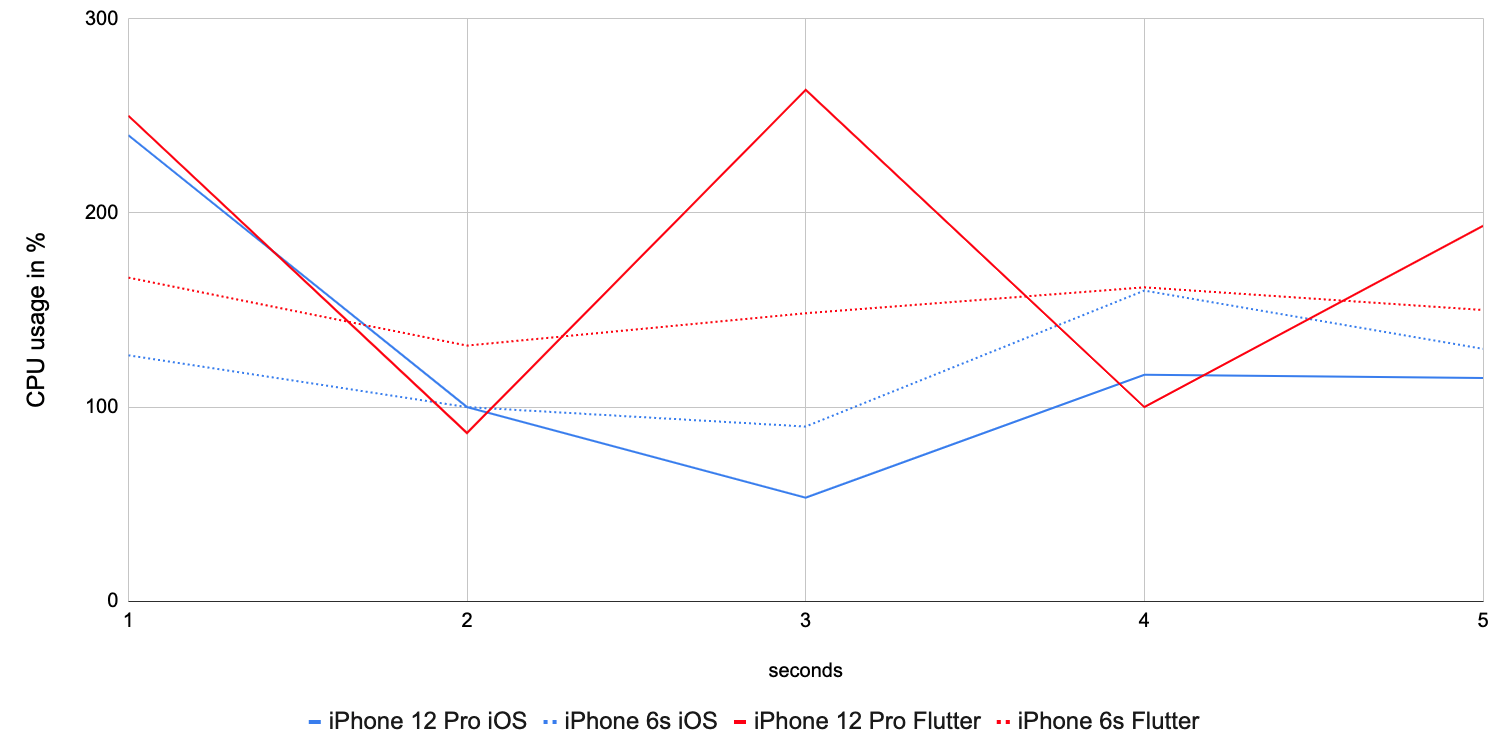
\includegraphics[width=\linewidth]{images/performance_results/app_start/avg_cpu_usage_app_start.png}
    \caption{Averaged CPU Usage App Start}
    \label{fig:avg_cpu_usage_app_start}
\end{figure}

\begin{figure}[!h]
    \centering
    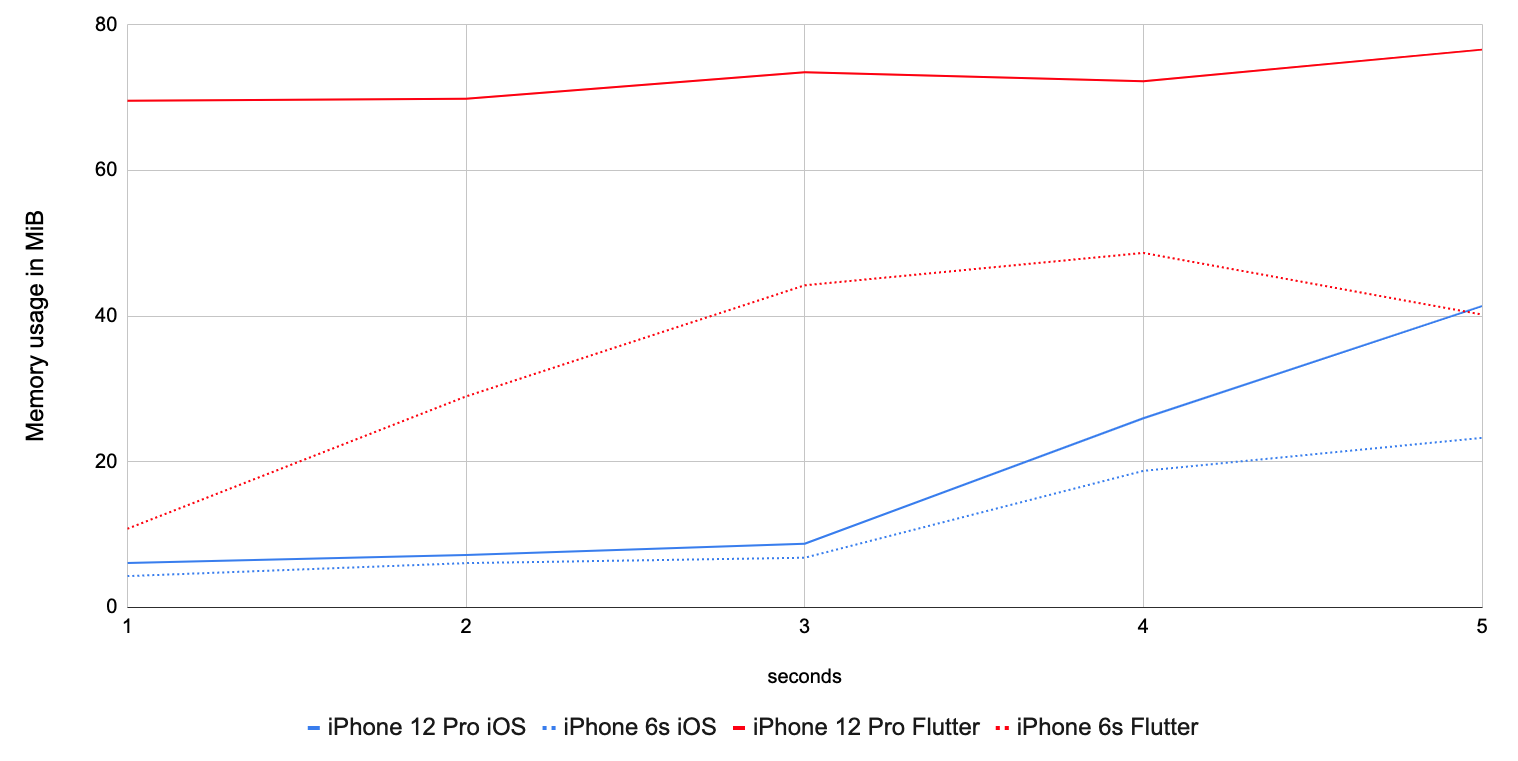
\includegraphics[width=\linewidth]{images/performance_results/app_start/avg_memory_usage_app_start.png}
    \caption{Averaged Memory Usage App Start}
    \label{fig:avg_memory_usage_app_start}
\end{figure}

\begin{figure}[!h]
    \centering
    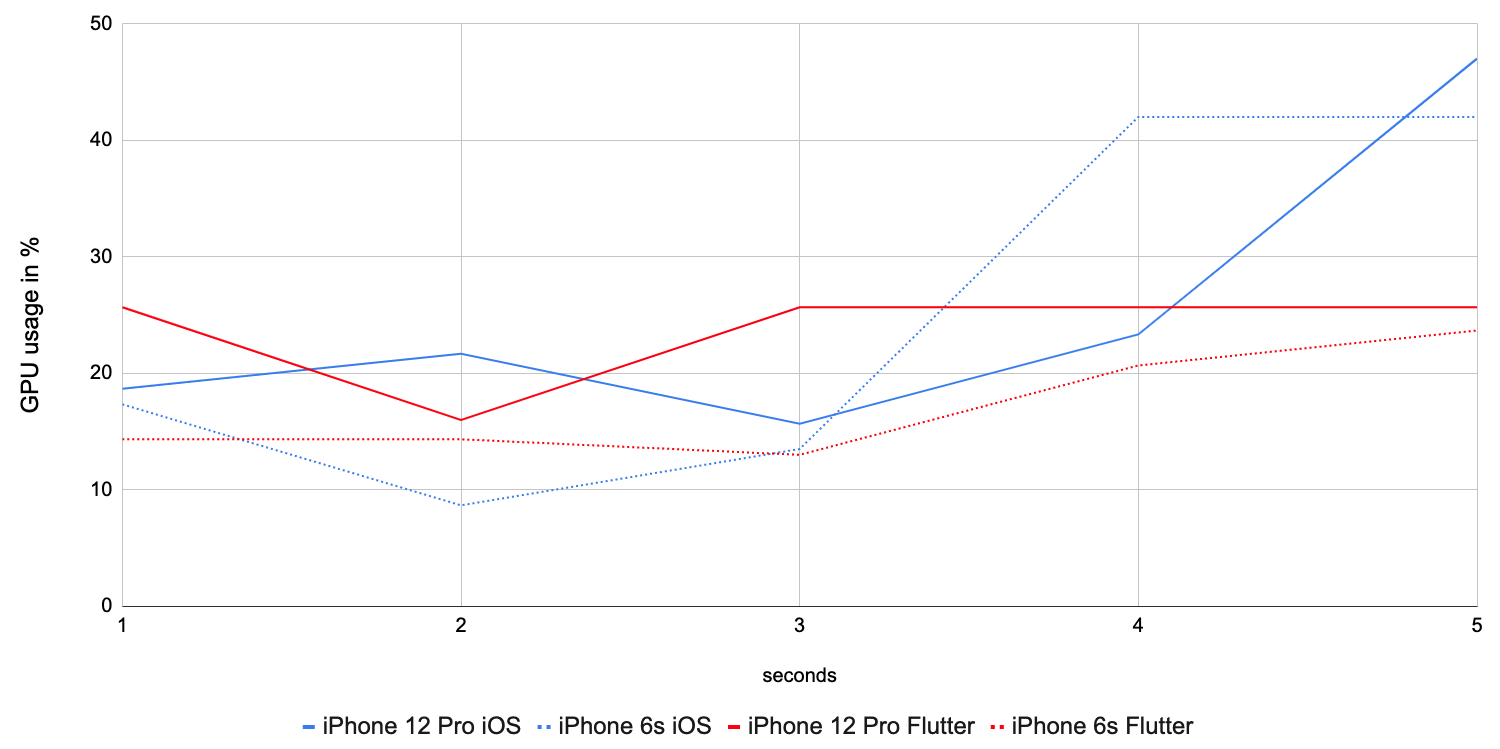
\includegraphics[width=\linewidth]{images/performance_results/app_start/avg_gpu_usage_app_start.png}
    \caption{Averaged GPU Usage App Start}
    \label{fig:avg_gpu_usage_app_start}
\end{figure}


\subsection{Detail View}
\begin{figure}[!h]
    \centering
    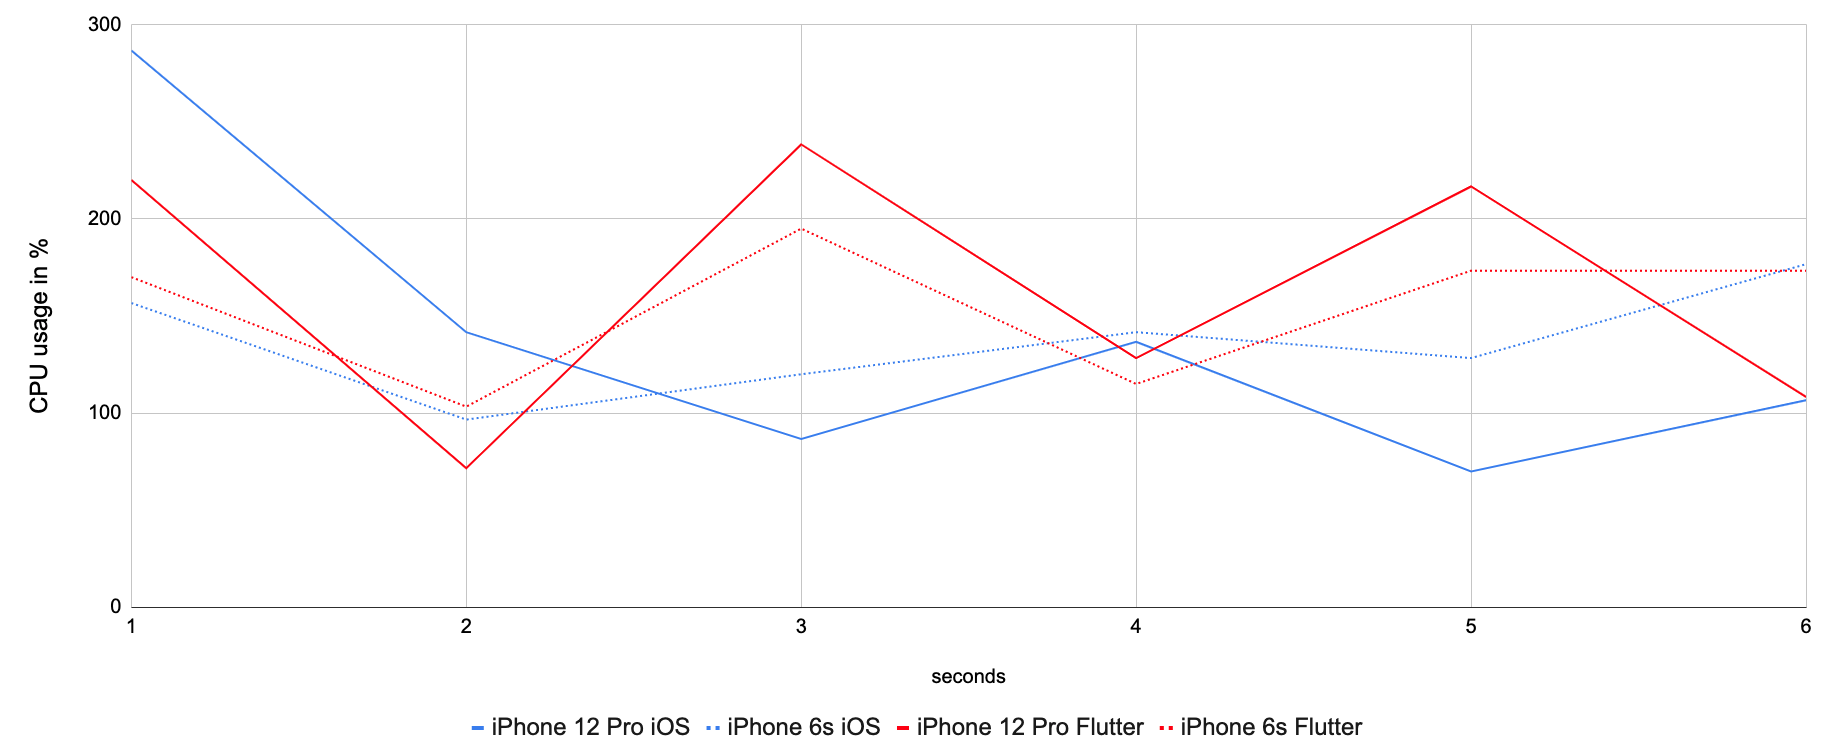
\includegraphics[width=\linewidth]{images/performance_results/detail_view/avg_cpu_usage_detail_view.png}
    \caption{Averaged CPU Usage Detail View}
    \label{fig:avg_cpu_usage_detail_view}
\end{figure}

\begin{figure}[!h]
    \centering
    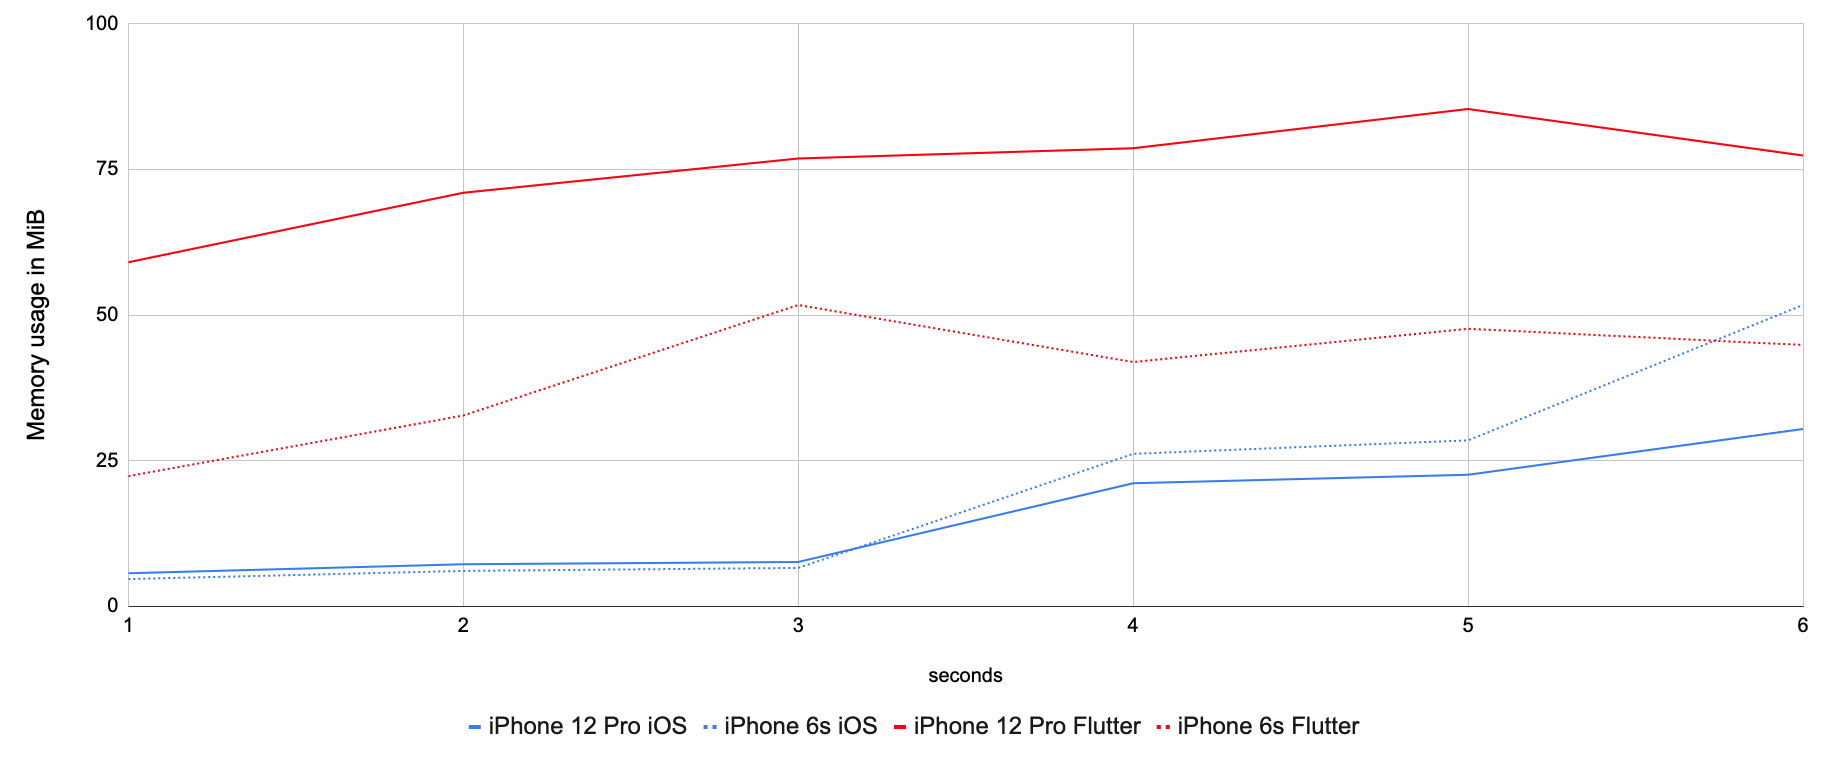
\includegraphics[width=\linewidth]{images/performance_results/detail_view/avg_memory_usage_detail_view.png}
    \caption{Averaged Memory Usage Detail View}
    \label{fig:avg_memory_usage_detail_view}
\end{figure}

\begin{figure}[!h]
    \centering
    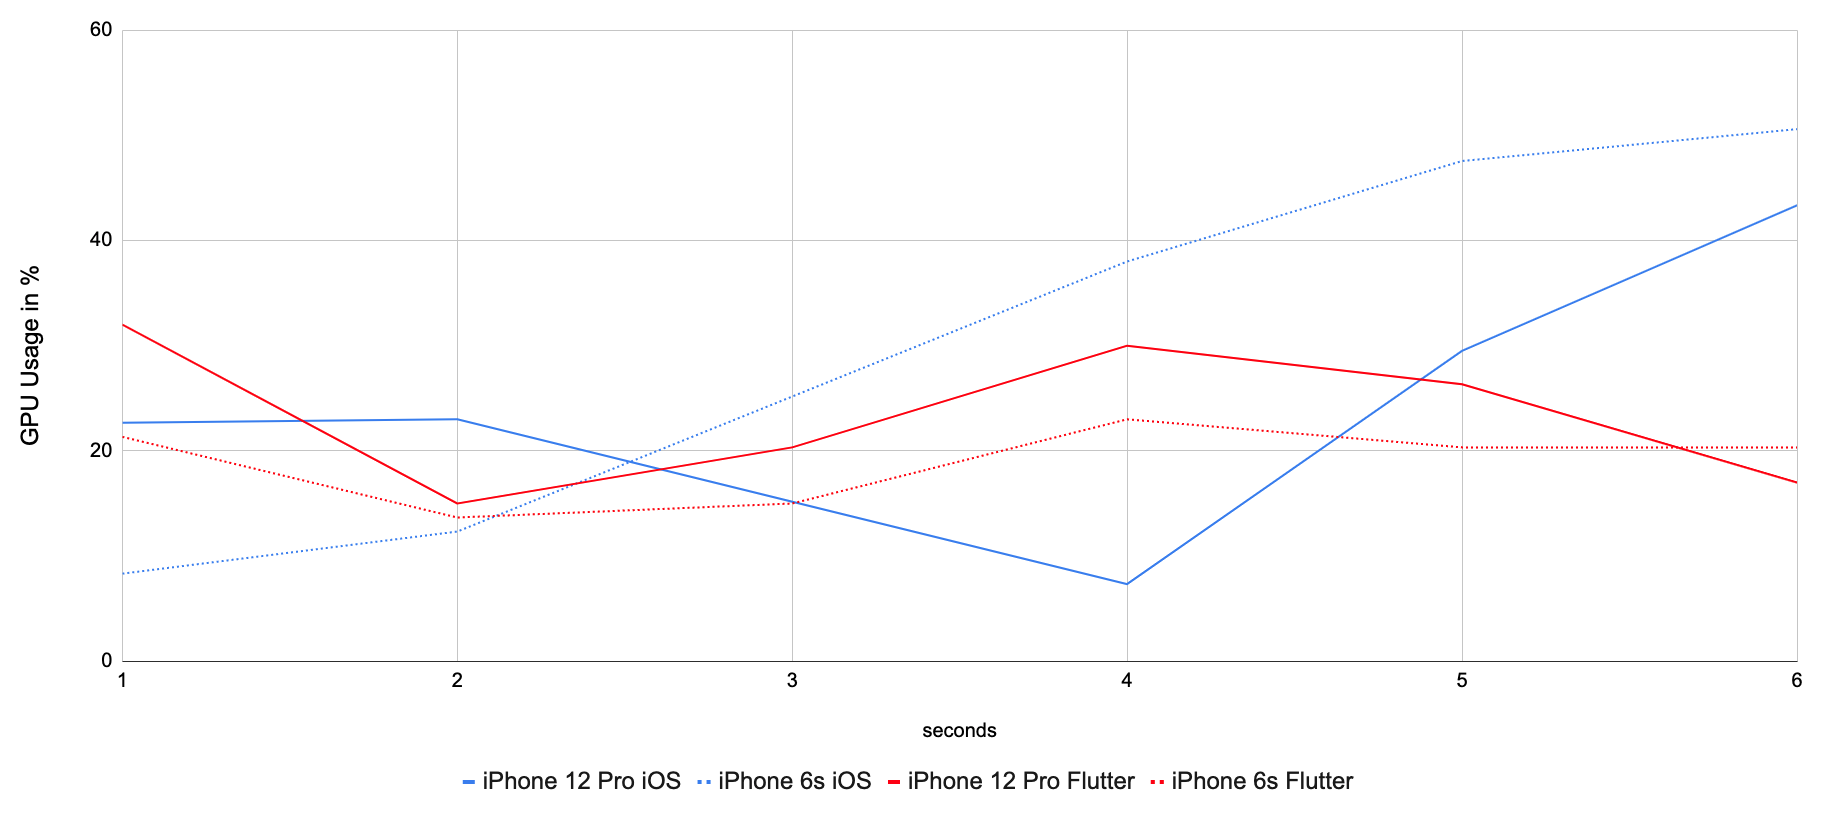
\includegraphics[width=\linewidth]{images/performance_results/detail_view/avg_gpu_usage_detail_view.png}
    \caption{Averaged GPU Usage Image Gallery}
    \label{fig:avg_gpu_usage_image_gallery}
\end{figure}



\subsection{Image Gallery}
\begin{figure}[!h]
    \centering
    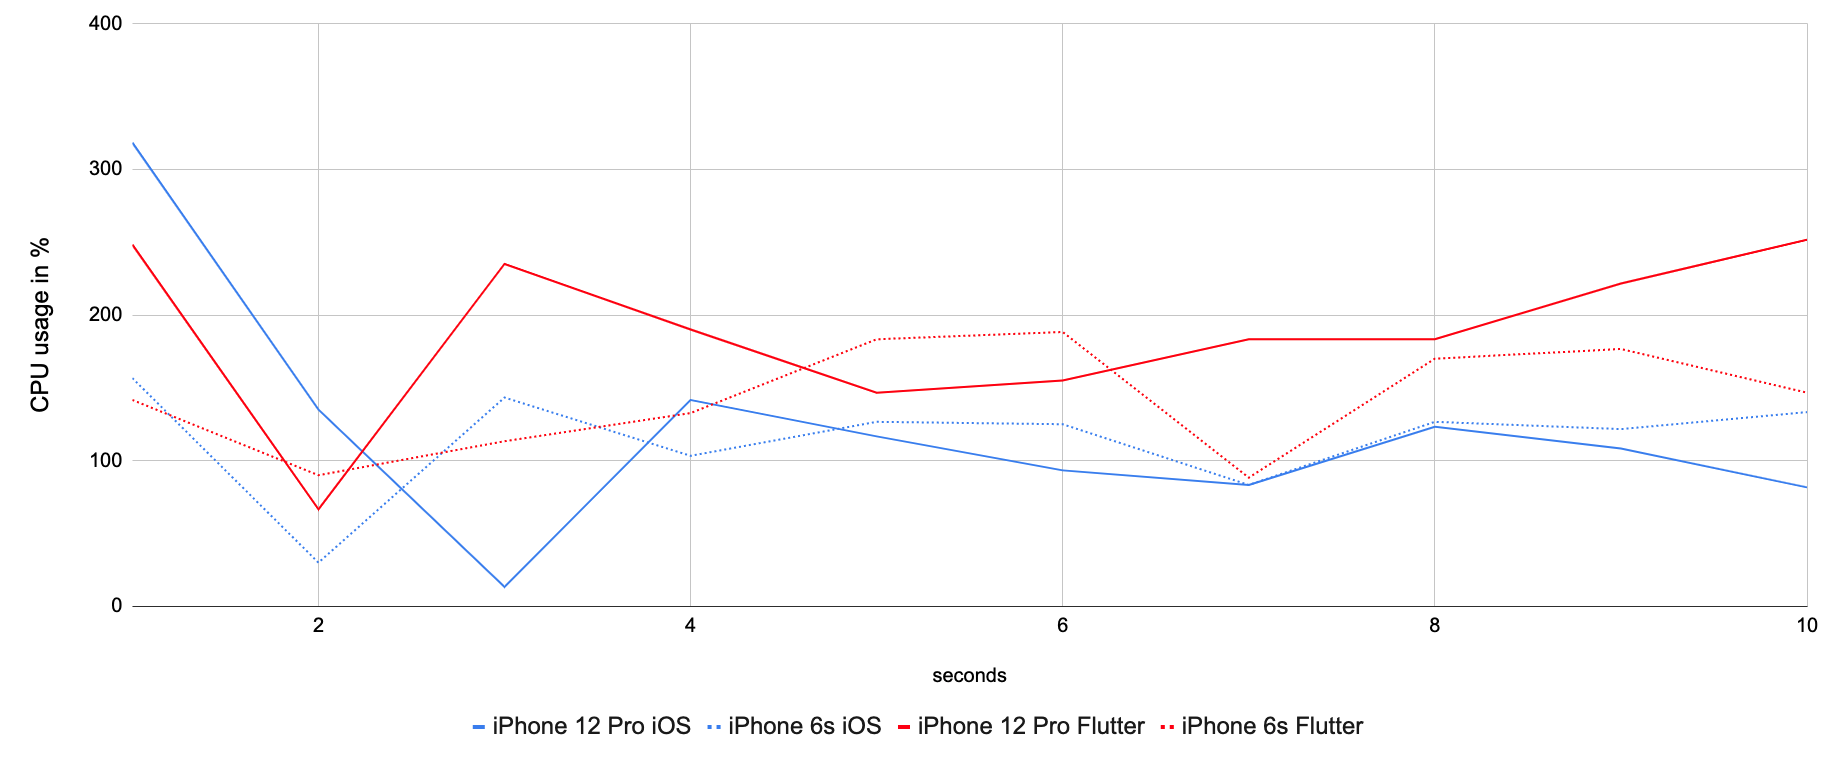
\includegraphics[width=\linewidth]{images/performance_results/image_gallery/avg_cpu_usage_image_gallery.png}
    \caption{Averaged CPU Usage Image Gallery}
    \label{fig:avg_cpu_usage_image_gallery}
\end{figure}

\begin{figure}[!h]
    \centering
    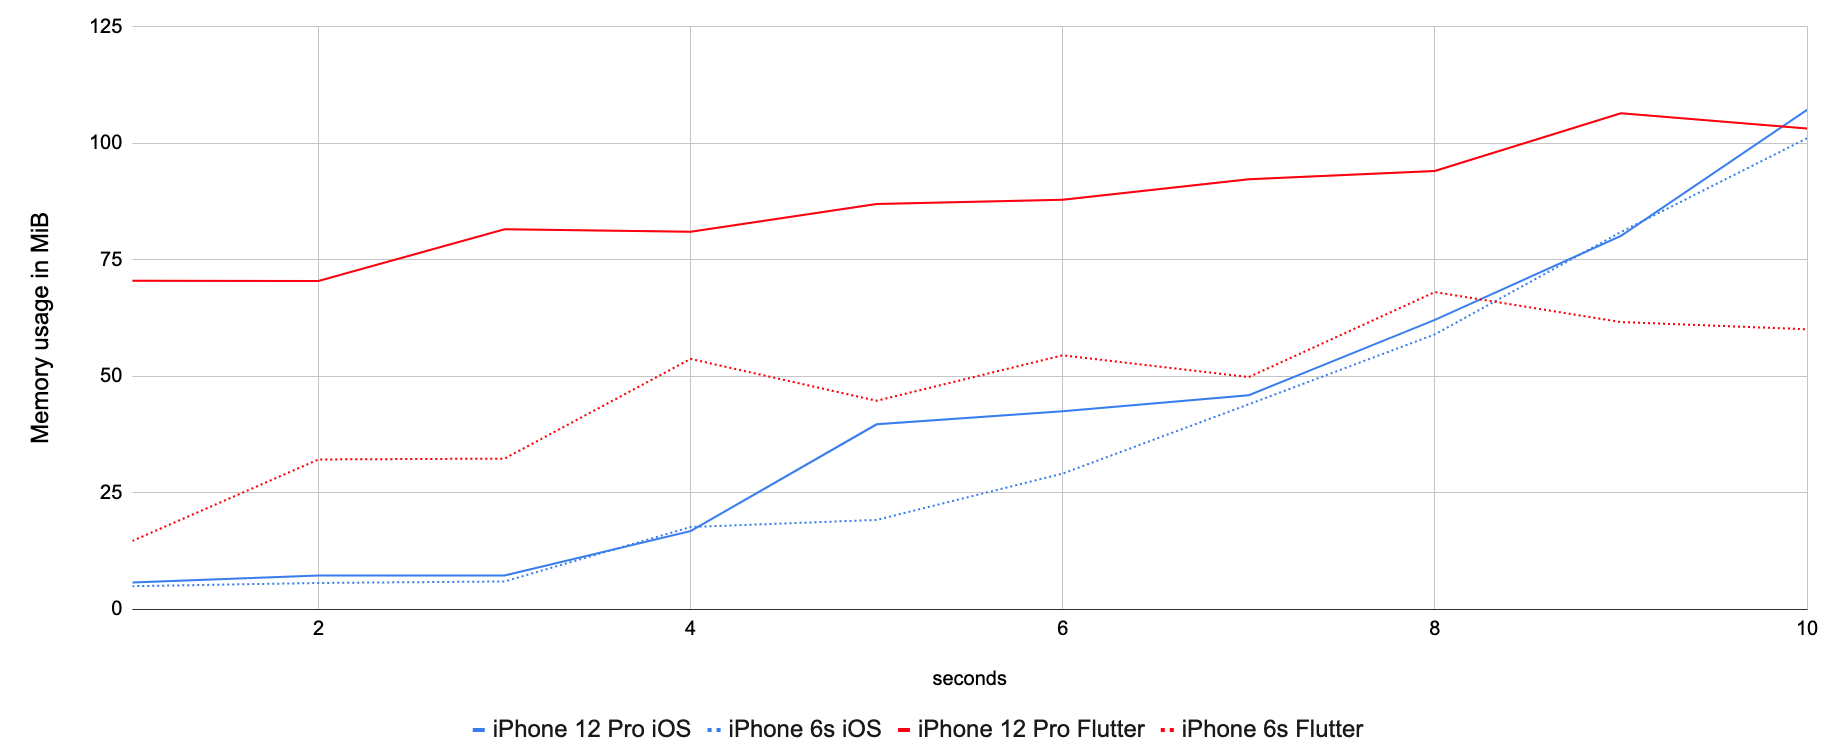
\includegraphics[width=\linewidth]{images/performance_results/image_gallery/avg_memory_usage_image_gallery.png}
    \caption{Averaged Memory Usage Image Gallery}
    \label{fig:avg_memory_usage_image_gallery}
\end{figure}

\begin{figure}[!h]
    \centering
    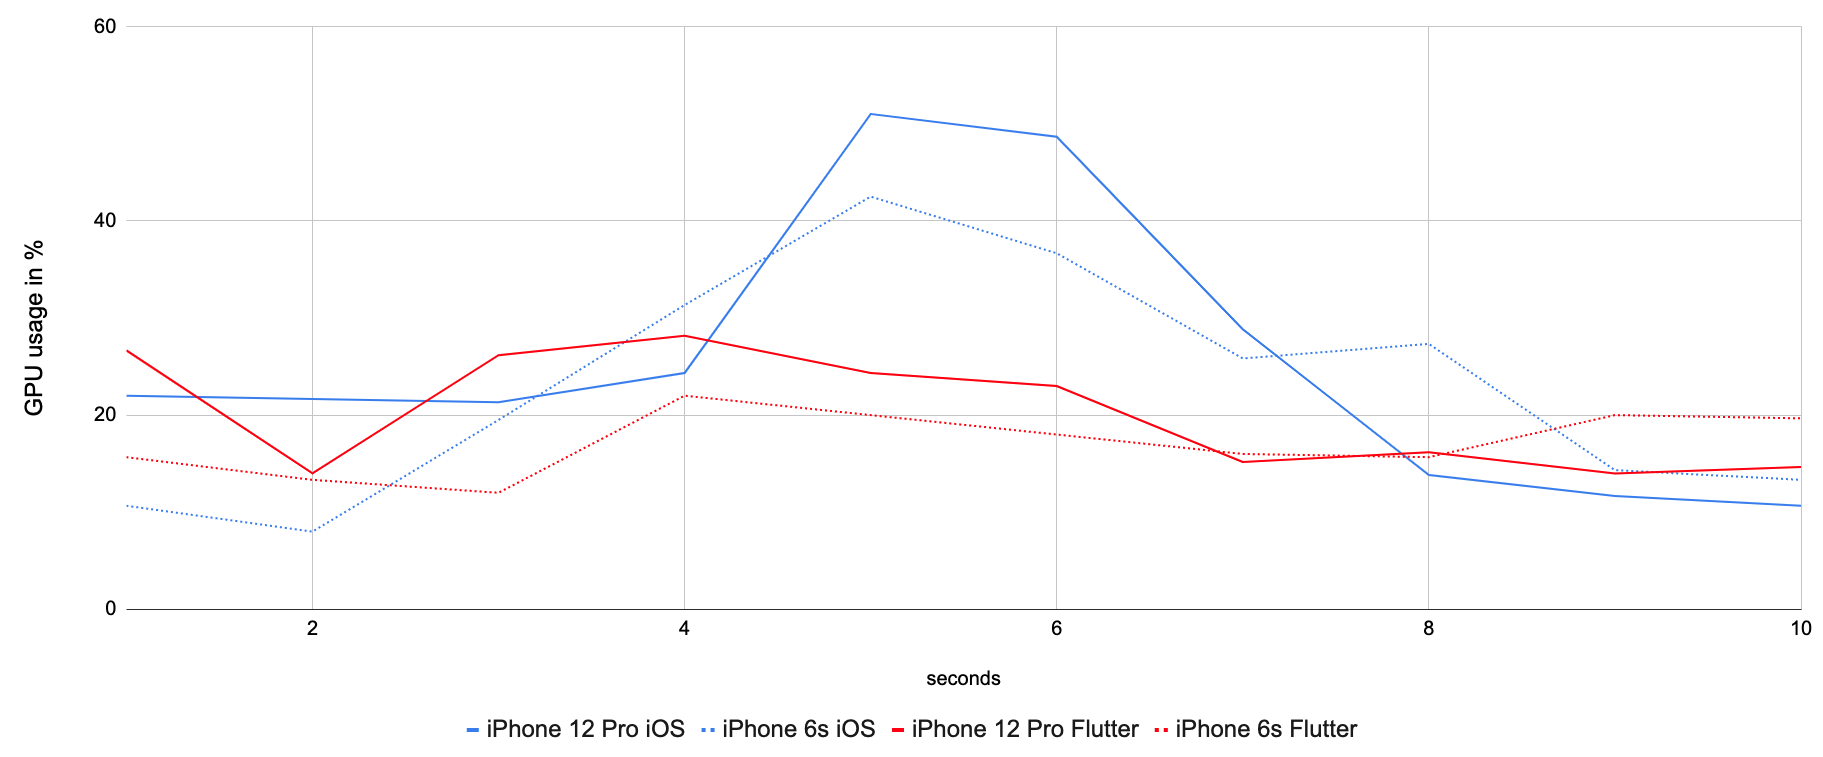
\includegraphics[width=\linewidth]{images/performance_results/image_gallery/avg_gpu_usage_image_gallery.png}
    \caption{Averaged GPU Usage Image Gallery}
    \label{fig:avg_gpu_usage_detail_view}
\end{figure}


\subsection{Scrolling}

\begin{figure}[!h]
    \centering
    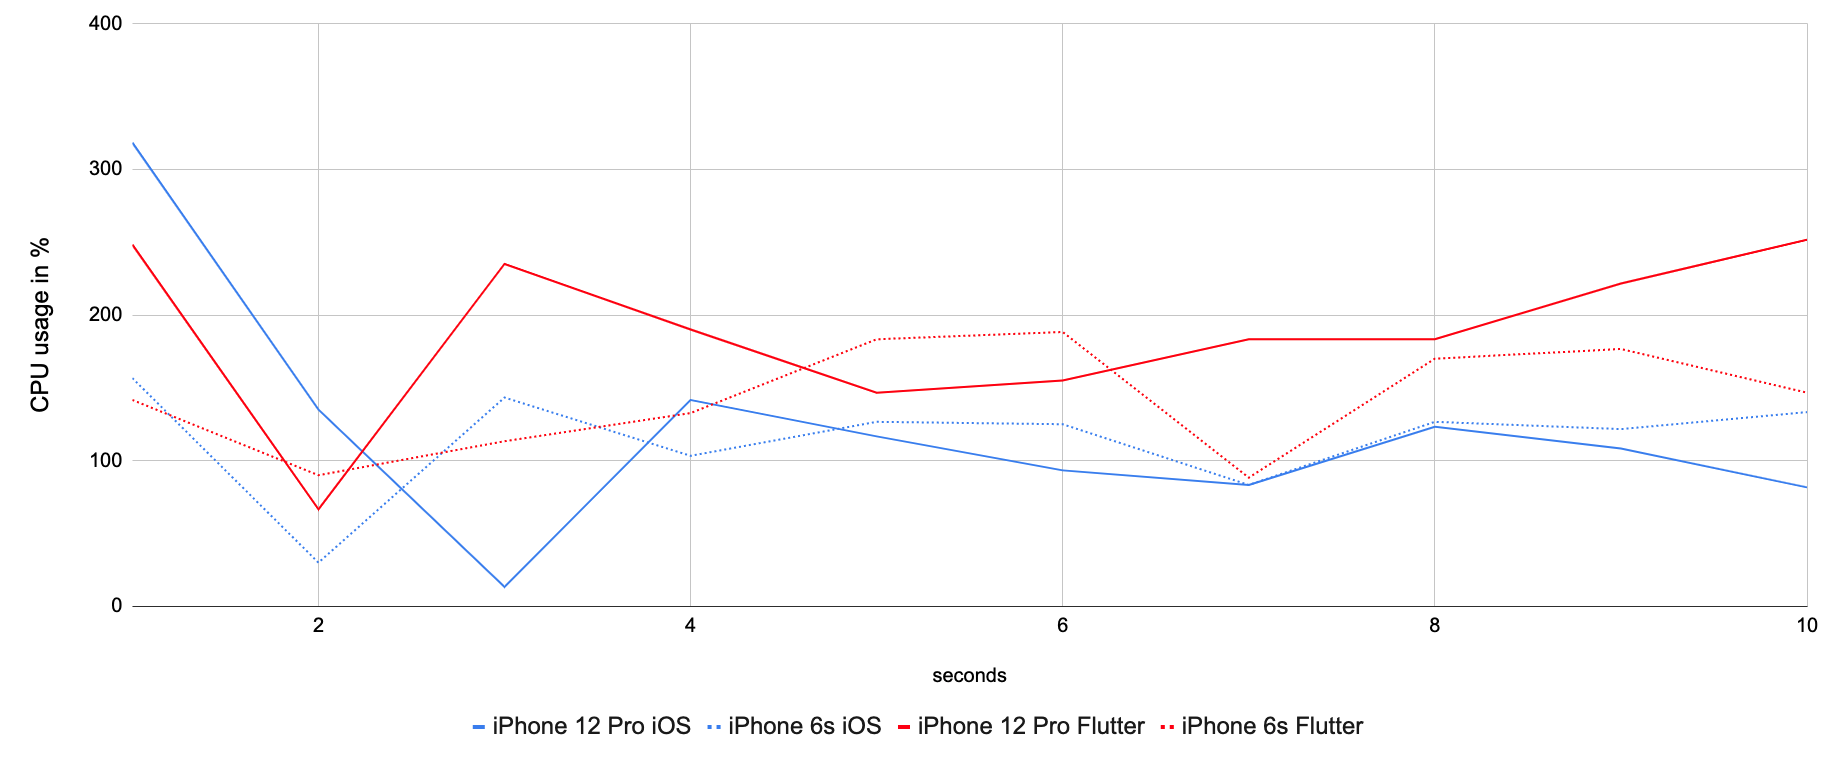
\includegraphics[width=\linewidth]{images/performance_results/image_gallery/avg_cpu_usage_image_gallery.png}
    \caption{Averaged CPU Usage Scrolling}
    \label{fig:avg_cpu_usage_scrolling}
\end{figure}

\begin{figure}[!h]
    \centering
    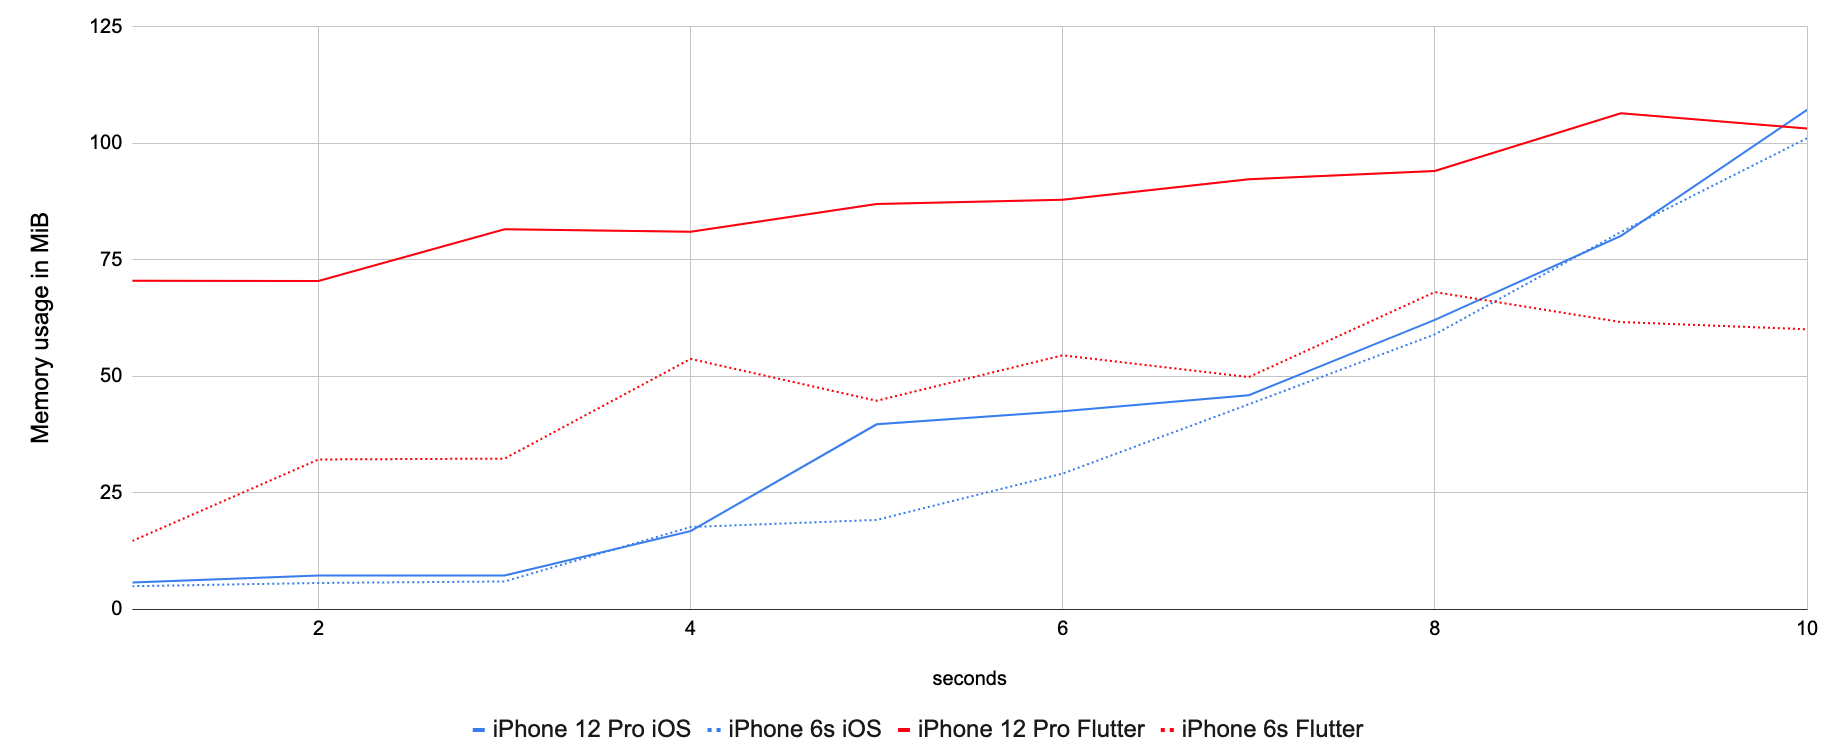
\includegraphics[width=\linewidth]{images/performance_results/image_gallery/avg_memory_usage_image_gallery.png}
    \caption{Averaged Memory Usage Scrolling}
    \label{fig:avg_memory_usage_scrolling}
\end{figure}

\begin{figure}[!h]
    \centering
    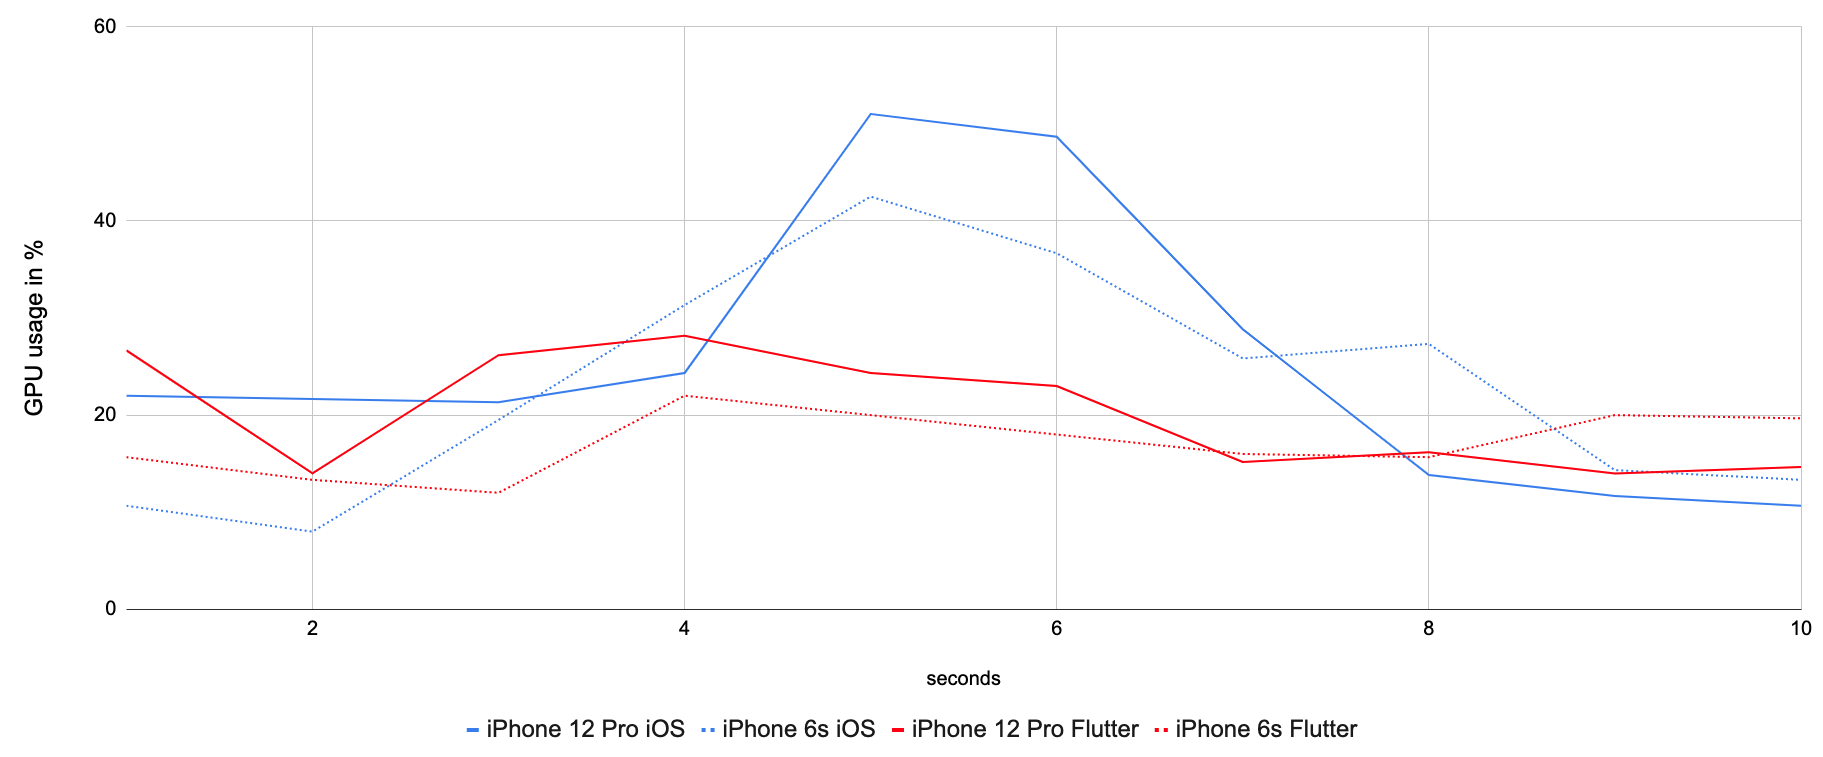
\includegraphics[width=\linewidth]{images/performance_results/image_gallery/avg_gpu_usage_image_gallery.png}
    \caption{Averaged GPU Usage Scrolling}
    \label{fig:avg_gpu_usage_scrolling}
\end{figure}

\section{Interview Transcriptions}

\textbf{A:} Author\\
\textbf{I:} Interviewee

\subsection{Interview 1}
\textbf{Date:} 07.04.21\\
\textbf{Job title:} Junior UI/UX Designer\\
\textbf{Years working in mobile industry:} 1,5\\
\textbf{Experience with Kickdown App}: Has heard of the app, but never used it\\

\begin{myparindent}{0pt}

\textbf{A:} Öffne Kickdown A und suche den weißen Jaguar aus Böblingen. Dann einmal bitte Kickdown B öffnen und den Golf 1 Cabrio aus Hamburg finden. Konntest du irgendwelche Unterschiede feststellen zwischen den beiden Apps im nachhinein?

\textbf{I:} Also eigentlich sieht es vom UI sehr gleich aus und beim Scrollen konnte ich auch nichts feststellen. 

\textbf{A:} Ja, alles gut. Und wenn du dich entscheiden müsstest zwischen eine der beiden Nutzererfahrungen, welche wäre das? "Beide sind" gleich ist auch ok.

\textbf{I:} Also ich kann es nicht sagen, welche ich besser finde. Finde es schwierig. 

\textbf{A:} Das ist auch in Ordnung. Ist auch eine gute Antwort. Dann würde ich dich bitten B zu öffnen und dir da dein Lieblingsauto rauszusuchen. Dann kannst du mal rauf tappen. Jetzt kannst du bieten und dort deine Lieblingszahl eingeben.

\textbf{I:} Hier kommt jetzt ein Dialog.

\textbf{A:} Das ist weil du dich nicht angemeldet hast. Das ist in Ordnung. Magst du das gleiche Prozedere bitte einmal für A wiederholen 

\textbf{I:} Hier ist jetzt eine andere Transition. Die fand ich bei B irgendwie cooler. Das war so eine Hero Animation. Aber das sheet kommt hier smoother hoch. Das war bei der anderen so abgehackt. Lass mich das nochmal in der anderen App ansehen. Ja, da ist so eine Lücke beim Hochfahren. Die Transition von dem Action Sheet ist schneller als die von der Tastatur und dadurch kommt diese Lücke zustande

\textbf{A:}  Wenn du nochmal insgesamt überlegst, also die Transition auf den Screen und dann das Hochfahren des Screens. Wie würdest du diesen ganzen Flow bewerten, wenn du dich zwischen den beiden Apps entscheiden müsstest?

\textbf{I:} Ich fand die Transition bei A besser, aber die Bieten UI bei B besser. Daher würde ich insgesamt sagen beide sind gleich. Aber das ist schwierig.

\textbf{A:} Ok. Dann öffne doch bitte noch einmal Kickdown A. Und von dem ersten Auto einmal das Bild raussuchen, wo die ganzen Zettel zu sehen sind. Du kannst die Gallery öffnen, indem du auf das Bild tippst. Da hast du es auch schon.  

\textbf{I:} Oh, das sind wirklich viele Zettel 

\textbf{A:} Und in der B kannst du dir nochmal noch das 2. Auto vornehmen und das Bild mit den Zetteln  heraussuchen. Es sind nicht ganz so viele, aber hier solltest du einen "Oldheimer Gutachten" sehen können. 

\textbf{I:} Hier ist er. Jetzt fragst du mich bestimmt wieder, welches ich besser fand. 

\textbf{A:} So langsam erkennst du glaube ich auch den Aufbau dieses Interviews. Konntest du zwischen den beiden Apps irgendwelche Unterschiede feststellen in Bezug auf die Usability?

\textbf{I:} Also das Öffnen der Gallerie funktioniert bei beiden gleich. Das kommt so von unten nach oben rein. Beim Swipen habe ich das Gefühl, dass es bei  B erst noch lädt. Wobei das wird animiert oder?

\textbf{A:} Genau, das ist eine Fade Animation.

\textbf{I:} Achso, das finde ich eigentlich schöner. Und sonst finde ich auch keine Unterschiede beim Zoomen oder wenn ich schnell swipe. 

\textbf{A:} Dann habe ich nochmal einen letzten Use Case den wir nochmal durchgehen können. Und zwar, wenn du wieder App B öffnest und dort die Mehr Seite öffnest und dort Tracking aktivierst. Und dann kannst du einmal auf Datenschutz tippen. Das gleiche kannst du nochmal bitte für A machen. Du kannst dir eine andere Seite raussuchen, z.B. Impressum. 

\textbf{I:} Also bei der App A steht "Fertig" und bei der App B steht "Schließen". Ansonsten sieht das gleich aus.

\textbf{A:} Und beim Switch, erkennst du da irgendwelche Unterschiede?

\textbf{I:} Ne, also die sind auch genau gleich

\textbf{A:} Also dann konntest du hier insgesamt auch keinen Unterschied feststellen?

\textbf{I:} Ne.

\textbf{A:} Ok - vielen Dank!


\subsection{Interview 2}
\textbf{Date:} 07.04.21\\
\textbf{Job title:} UI/UX Designer\\
\textbf{Years working in mobile industry:} 8\\
\textbf{Experience with Kickdown App}: supported conceptual development of application\\

\textbf{A:}  Kannst du einmal bitte Kickdown A öffnen und den weißen Jaguar aus Böblingen heraussuchen. Und dann würde ich dich bitten in der App B den Golf 1 Cabrio aus Hamburg herauszusuchen

\textbf{I:} Hab ich.

\textbf{A:} Perfekt. Konntest du beim Öffnen der App und beim Scrollen irgendwelche Unterschiede feststellen?

\textbf{I:} Also in App B sind die Abstände vom Countdown Label etwas anders als in der Original App. Das Spacing zwischen den Zahlen ist etwas größer. Aber sonst sind sie wirklich sehr gleich. 

\textbf{A:} Und wenn du dich zwischen den beiden Apps für eine entscheiden müsstest, welche wäre das dann?

\textbf{I:} Das kann ich nicht sagen. Ich finde beides sehr ähnlich.

\textbf{A:} Kannst du bitte einmal in App B ein Auto deiner Wahl aussuchen und kannst auf das Auto bieten. Du bist nicht eingeloggt von daher sollte nichts passieren. Wenn du durch bist, kannst du das gleiche noch einmal in App A machen. Konntest du irgendwelche Unterschiede feststellen? Sowohl bei der Transition auf den Detail View als auch beim Bieten selbst?

\textbf{I:} Da konnte ich im ersten Moment nichts feststellen. Kann ich das ganze auch nochmal durchspielen?

\textbf{A:} Klar. Du kannst dir beide Apps nochmals genauer anschauen.

\textbf{I:} Ok, wenn ich jetzt nochmal darüber schaue, ist die Animation hier [Bottom Sheet zum Bieten] bei A flüssiger. Also würde ich sagen: A.

\textbf{A:} Ok, perfekt. Du bist jetzt noch in A richtig?

\textbf{I:} Ja

A. Dann öffne bitte einmal die Übersichtsseite und von dem ersten Auto das Bild heraussuchen, wo extrem viele Zettel zu sehen sind. Dafür kannst du auch die Gallerie öffnen.

\textbf{I:} Hier. 

\textbf{A:} Sehr gut. Und in B kannst du von dem 2. Auto das Bild heraussuchen, wo ebenfalls viele, aber nicht ganz so viele Zettel zu sehen sind. Dort solltest du ein "Oldheimer Gutachten" sehen können.

\textbf{I:} Ah ok. Das müsste es sein - ja. 

\textbf{A:} Konntest du bei diesem Use Case irgendwelche Unterschiede feststellen?

\textbf{I:} Garnicht

\textbf{A:} Garnicht?

\textbf{I:} Wenn ich nochmal schaue. Das Öffnen der Gallerie ist gleich. Ich kann hier bei B noch weiter reinzoomen. Bei B kommen die Bilder ein bisschen verzögert reinanimiert. Aber da kann ich sonst keine Unterschiede feststellen, was kaum auffällt. Also, da kann ich mich nicht entscheiden.

\textbf{A:} Alles klar. Dann kommen wir zum nächsten Use Case. Du darfst einmal in App B das Tracking einschalten. Das kannst du über die "Mehr"-Seite machen. Und jetzt einmal "About Kickdown" öffnen. Du kannst die Seite wieder schließen. Das war es auch schon. Nun magst du das gleiche nochmal für A wiederholen. Du kannst auch eine andere Seite öffnen.

\textbf{I:} Du fragst mich bestimmt, ob ich irgendwelche Unterschiede feststellen konnte.

\textbf{A:} Genau. 

\textbf{I:} Also, da konnte ich jetzt absolut nichts erkennen.

\textbf{A:} Auch beim Switch betätigen?

\textbf{I:} Alles gleich.

\textbf{A:} Das waren jetzt auch schon alle Use Cases.


\subsection{Interview 3}
\textbf{Date:} 07.04.21\\
\textbf{Job title:} Junior UI/UX Designer\\
\textbf{Years working in mobile industry:} 8\\
\textbf{Experience with Kickdown App}: conceptual development of application\\

\textbf{A:} Du kannst gerne einmal Kickdown B öffnen und dort den weißen Jaguar aus Böblingen heraussuchen 

\textbf{I:} Da ist er. 

\textbf{A:} Sehr gut. Nun bitte ich dich einmal in Kickdown A den Golf 1 Cabrio aus Hamburg zu finden. 

\textbf{I:} Das müsste er sein. 

\textbf{A:} Super. Nur vom App Start und Scrollen. Konntest du irgendwelche Unterschiede feststellen?

\textbf{I:} Nein.

\textbf{A:} Das heißt du würdest auch dementsprechend keine der beide Erfahrungen präferieren?

\textbf{I:} Genau.

\textbf{A:} Dann - du bist ja jetzt in Kickdown A - würde ich dich bitten auf den Überblick zu gehen und dort ein Auto deiner Wahl auszusuchen. Dieses kannst du dann einmal Öffnen und dort auf das Auto bieten. Du kannst irgendeinen Betrag eingeben. Du bist auch nicht angemeldet, also wird da auch nichts gesendet. 
Super - vielen Dank. Du kannst dir gerne einmal in der App B nun ein anderes Auto raussuchen und dort bieten.

\textbf{I:} Ok. 

\textbf{A:} Sehr gut. Vielen Dank. Dann jetzt einmal wieder die Frage: Konntest du zwischen den beiden Apps in diesem Use Case irgendwelche Unterschiede feststellen?

\textbf{I:} Bei A hat man bei der Screen Transition die typische Detail Animation. Bei der anderen ist das irgendeine andere Animation. Ansonsten sieht man bei A auch die bottom sheet Animation, wo der Hintergrund so wegfährt. Bei B ist das nicht ganz wie im Original. Und bei B ist die Animation nicht so schön. Ich glaube es liegt einfach an der Animationskurve. Die Animationskurve ist einfach linear.

\textbf{A:} Wenn du dich entscheiden müsstest, welche wäre das hier?

\textbf{I:} Dann wähle ich Variante A.

\textbf{A:} Ich bitte dich nochmal in App B das erste Auto auszuwählen und dort das Bild auszuwählen, wo extrem viele Zettel zu sehen sind. 

 \textbf{I:} Das ist hier - Bild 7. 

\textbf{A:} Cool. Dann kannst du noch einmal in die App A springen und dort beim 2. Auto das Bild heraussuchen, in dem ebenfalls viele Zettel zu sehen sind, allerdings nicht so viele. Da müsstest du ein "Oldheimer Gutachten" sehen.

\textbf{I:} Das meinst du, oder?

\textbf{A:} Konntest du in der User Experience irgendwelche Unterschiede feststellen

\textbf{I:} Also in A ist das erste Bild kurz weg. 

\textbf{A:} Genau. Das ist tatsächlich bei beiden Apps so, da die Bilder von der API nochmals neu nachgeladen werden.

\textbf{I:} Ansonsten konnte keine Unterschiede feststellen.

\textbf{A:} Ok. Dann bitte ich dich noch einmal in App A zu gehen und dort einmal Tracking einzuschalten. Und dort einmal "About Kickdown" zu öffnen. 

\textbf{I:} Und dann?

\textbf{A:} Das war es schon. Das Gleiche kannst du nochmal bitte für B machen. Du kannst natürlich noch eine andere Seite öffnen - z.B. Impressum.
Konntest du da irgendwelche Unterschiede feststellen.

\textbf{I:} Kann ich mir das nochmal genauer ansehen?

\textbf{A:} Ja, klar.

\textbf{I:} Das fühlt sich für mich beides doch sehr ähnlich an. Ich glaube der Font bei der Flutter App ist nicht der Originale. Also er sieht für mich auch nach einem SF Font aus.

\textbf{A:} Ja, ich glaube ich habe nicht alle Fonts importiert.

\textbf{I:} Ah ja. 

\textbf{A:} Präferierst du eine der beiden User Experiences?

\textbf{I:} Das kann ich dir nicht sagen

\textbf{A:} Ne, das ist auch in Ordnung. Danke Dir.

\subsection{Interview 4}
\textbf{Date:} 07.04.21\\
\textbf{Job title:} Senior iOS Software Engineer\\
\textbf{Years working in mobile industry:} 11\\
\textbf{Experience with Kickdown App}: co-developed the iOS application\\


\textbf{A:} Du darfst bitte einmal die Kickdown app A öffnen und auf der Übersichtsseite den weißen Jaguar aus Böblingen raussuchen

\textbf{I:} Ah, da ist er.

\textbf{A:} Dann bitte ich dich noch einmal in App B den Golf 1 Cabrio aus Hamburg zu finden. 

\textbf{I:} Die App unterstützt auf jeden Fall nicht Dynamic Type. 

\textbf{A:} Konntest du zwischen den beiden Apps irgendwelche Unterschiede in der User Experience feststellen?

\textbf{I:} Die App B scheint ein bisschen länger zu laden und Dynamic Type wird wie gesagt nicht unterstützt. Ansonsten ist das sehr gleich für mich. 

\textbf{A:} Ok. Und wenn du dich für eine der beiden Apps entscheiden müsstest aus User Experience Sicht?

\textbf{I:} Dann nehme ich natürlich A wegen der Dynamic Type Unterstützung. 

\textbf{A:} Sehr gut. Dann kannst du einmal bitte in App B ein Auto deiner Wahl raussuchen. 

\textbf{I:} Dann nehmen wir doch den Porsche 911.

\textbf{A:} Und kannst dort einmal bieten. Du kannst da irgendeine Zahl eingeben. Das Angebot wird nicht abgeschickt, da du noch nicht angemeldet bist. Ok - danke! 
Dann kannst du das Gleiche einmal bitte für App A durchführen. Du kannst dir auch gerne nochmal ein anderes Auto raussuchen. 

\textbf{I:} Ok, dann nehme ich mal diesen Porsche. 

\textbf{A:} Danke. Das war dann auch der nächste Use Case. Jetzt wieder die Frage an dich: Konntest du irgendwelche Unterschiede feststellen?

\textbf{I:} Ja, also die Transition bei der App ist auf jeden Fall schöner. Das andere ist eher langweilig.

\textbf{A:} Konntest du bei der Animation sonst noch irgendetwas feststellen beim Bieten?

\textbf{I:} Ist mir jetzt erstmal nichts aufgefallen. Lass mich nochmal schauen. Ah doch, also die Animation bei A fühlt sich natürlicher an. Die Transition bei B ist etwas schöner. Aber das Bottom Sheet ist dafür nativer bei App A. Daher würde ich mich in dem Fall auch für A entscheiden. 

\textbf{A:} Dann kannst du bitte einmal App A öffnen, auf das 1. Auto tippen und dort das Bild raussuchen, wo ganz viele Zettel zu sehen sind. 

\textbf{I:} Das hier meinst du?

\textbf{A:} Ja, richtig. Dann kannst du bitte in App B das 2. Auto raussuchen und das Bild finden, wo auch Zettel, allerdings einige weniger zu sehen sind. 

\textbf{I:} Das hier?

\textbf{A:} Top. Dann wieder die Frage an dich, ob du hier irgendwelche Unterschiede feststellen konntest. 

\textbf{I:} Hier bei App B sieht man die Status Bar nicht - das ist natürlich keine gute User Experience. Sonst Beim Swipen und Zoomen fällt mir nichts auf. 

\textbf{A:} Wenn du dich hier wieder für eine der beiden entscheiden müsstest, welche wäre das dann?

\textbf{I:} Dann würde ich hier wieder A wählen. 

\textbf{A:} Ok. Dann haben wir noch einen letzten Use Case, den wir gemeinsam durchgehen können. Magst du dazu bitte einmal Kickdown B öffnen und dort auf der Mehr Seite das Tracking einschalten. 

\textbf{I:} So.

\textbf{A:} Genau - das war's. Das Ganze kannst jetzt noch einmal bitte für App A ausführen. Perfekt - vielen Dank. Waren da für dich irgendwelche Unterschiede festzumachen?

\textbf{I:} Also hier sieht das für mich sehr gleich aus. Da kann ich nichts erkennen. 

\textbf{A:} Dementsprechend präferierst du auch keine der beiden Nutzererfahrungen?

\textbf{I:} Nein. 

\textbf{A:} Cool - danke Dir.


\subsection{Interview 5}
\textbf{Date:} 08.04.21\\
\textbf{Job title:} iOS Software Engineer\\
\textbf{Years working in mobile industry:} 8\\
\textbf{Experience with Kickdown App}: has heard of app, but never used it before\\

\textbf{A:} Alles klar. Dann lass uns doch direkt mit dem ersten Use Case starten. Öffne bitte einmal Kickdown B und suche dort nach dem weißen Jaguar aus Böblingen. 

\textbf{I:} Den hier meinst du?

\textbf{A:} Yes. Dann magst du einmal bitte Kickdown A öffnen und dort den schwarzen Golf 1 Cabrio aus Hamburg finden.

\textbf{I:} Hier ist er. 

\textbf{A:} Perfekt. Konntest du da irgendwelche Unterschiede zwischen den beiden Apps feststellen?

\textbf{I:} Lass mich nochmal ein bisschen durchscrollen. 

\textbf{A:} Klar. 

\textbf{I:} Das fühlt sich für mich sehr gleich an

\textbf{A:} Wenn du dich für eine der beiden Apps entscheiden müsstest, welche wäre das? Es ist auch ok zu sagen, dass du beide gleich gut findest. 

\textbf{I:} Ich empfinde beide für gleichwertig. 

\textbf{A:} Alles klar. Dann können wir einmal zum 2. Use Case übergehen. Dazu kannst du dir ein Auto deiner Wahl aussuchen in App A und dort Bieten. Du kannst irgendeine Zahl eingeben. Du bist nicht angemeldet und somit wird dein Angebot auch nicht abgeschickt.

\textbf{I:} Alright, dann holen wir uns doch den Porsche. 

\textbf{A:} Viel Erfolg! Top - dann kannst du das gleiche einmal bitte in App B durchführen. 

\textbf{I:} Der Font ist hier von dem Dialog auf jeden Fall nicht richtig. Das erkenne ich sofort. Das sieht nicht richtig aus für mich. 

\textbf{A:} Ah interessant. Gibt es sonst Unterschiede?

\textbf{I:} Das Bottom Sheet ist nicht Draggable in App B. Die Animation fühlt sich auch nicht nativ an. Aber das liegt nicht an Flutter. Das wurde dann einfach nicht genau gleich implementiert

\textbf{A:} Ok danke. Wenn du dich wieder für eine App entscheiden müsstest, welche wäre das?

\textbf{I:} Dann würde ich ganz klar sagen: A. 

\textbf{A:} Ok cool. Dann bitte ich dich bitten einmal App A zu öffnen und dort erste Auto auf der Überssichtsseite auszuwählen und dort das Bild mit den Sonnenschirmen zu finden.

\textbf{I:} Das meinst du?

\textbf{A:} Yes. Magst du nun bitte die App B öffnen und dort das 2. Auto auf der Überssichtsseite aussuchen und in der Gallerie das Bild finden, wo man das Nummernschild gut ablesen kann?

\textbf{I:} Hier.

\textbf{A:} Danke. Jetzt wieder die Frage: Konntest du irgendwelche Unterschiede feststellen?

\textbf{I:} Die funktionieren beide gleich. Das Swipen ist bei der Flutter App auch flüssig.

\textbf{A:} Also präferierst du auch keine der beiden Apps in diesem Fall?

\textbf{I:} Die sind beide gleich.

\textbf{A:} Top. Dann habe ich noch einen Use Case vorbereitet. Dafür kannst du in App B bleiben und bitte einmal auf der "Mehr"-Seite das Tracking einschalten und anschließend die "About Kickdown" Seite öffnen. 

\textbf{I:}: Ok. Ich muss immer schauen, ob die Seite "Bounce" hat. Das ist ganz wichtig. Aber die scheint einen guten "Bounce" zu haben.

\textbf{A:} Das war es auch schon. Das Ganze kannst du nun nochmals für Kickdown A wiederholen. 

\textbf{I:} Ok. Also hier öffnet sich die Webview auf jeden Fall gleich. Lass mich das nochmal prüfen. 

\textbf{A:} Klar.

\textbf{I:} Das ist wirklich gleich. 

\textbf{A:} Ok. Präferierst du in diesem Beispiel eine der beiden Apps von der User Experience?

\textbf{I:} Ne - die sind beide gleich. 

\textbf{A:} Cool - vielen Dank.

\end{myparindent}